\chapter{Introduction and Literature Review}

\begin{quote}
Chapter abstract goes here.
I should check if the concept of "Introduction \emph{and} Lit Review" is required.
Having an abstract for the introduction seems dumb, and I'm not sure I want a monolithic lit review up front.
\end{quote}

\section{Introduction}

We're talking about Choreographic Programming (CP).

\section{An illustrative example}

\Cref{fig:kvsenclave} shows an example choreography.
Probably a KVS variation.
Here we describe what it does and how to read it.

\begin{figure}[tbhp]\caption{Example Choreography: a key-value store}
  \begin{mdframed}
  \begin{tabular}{c c}
  \begin{minipage}{8.75cm}
    \inputminted[xleftmargin=10pt,linenos,fontsize=\scriptsize]{haskell}{figures/kvsenclave_a.hs.txt}
  \end{minipage}
  &
  \begin{minipage}{3.75cm}
    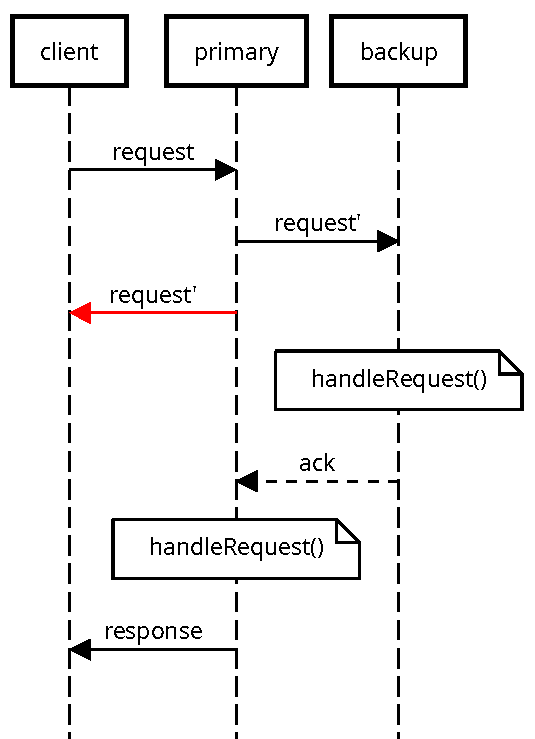
\includegraphics[width=4cm]{figures/seq2.pdf}
  \end{minipage} \\\\
  \multicolumn{2}{c}{\begin{minipage}{12.5cm}
  A key-value store with a backup server, written in \MultiChor.
           The backup server sends an acknowledgement message \textsf{ack} to the primary server
           if and only if \inlinecode{request} is a \inlinecode{Put}.
           The \inlinecode{broadcast} operator (line 19) ensures KoC
           so that the primary and backup servers are guaranteed to use the same case of \inlinecode{handleBackup},
           but it results in redundant communication (shown in red in the sequence diagram).
  \end{minipage}}\\\\
  \hline\\
  \begin{minipage}{8.75cm}
    \inputminted[xleftmargin=10pt,linenos,fontsize=\scriptsize]{haskell}{figures/kvsenclave_b.hs.txt}
  \end{minipage}
  &
  \begin{minipage}{3.75cm}
     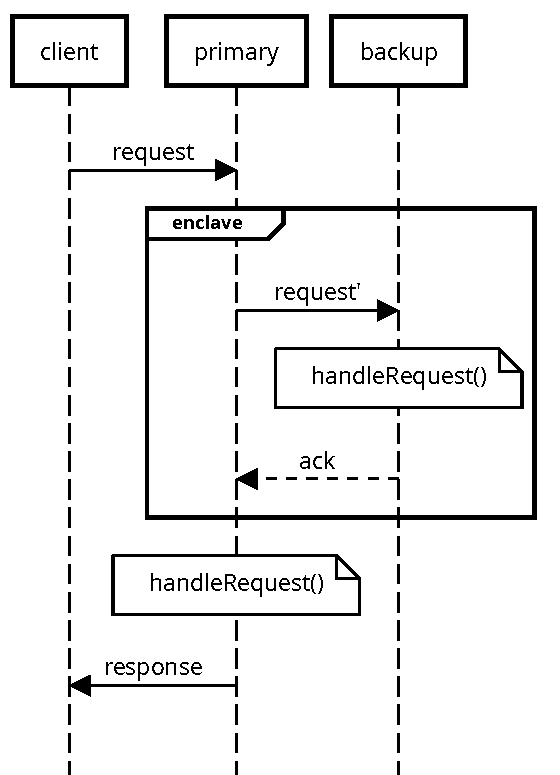
\includegraphics[width=4cm]{figures/seq3.pdf}
  \end{minipage} \\\\
  \multicolumn{2}{c}{\begin{minipage}{12.5cm}
  In this variation, the \inlinecode{enclave} operator eliminates the redundant communication.
           The enclaved sub-choreography is indicated by a box in the sequence diagram.
           On line~2, \inlinecode{@@ nobody} is \MultiChor idiom explained in \Cref{sec:membership}.
  \end{minipage}}
  \end{tabular}
  \label{fig:kvsenclave}
    %%\Description{In the top section, twenty four lines of Haskell code using the MultiChor library, with a UML sequence diagram of that program.
%%	The code defines a choreography called "kvs", and helper-functions "handleRequest" and "handleBackup".
%%	In the sequence diagram, first "client" sends "request" to "server",
%%	  then "server" sends "request-prime" to "client" and "backup",
%%	  then backup calls "handleRequest",
%%	  then backup may send "ack" to "server",
%%	  then server calls "handleRequest",
%%	  then server sends "response" to "client.
%%	The bottom sections shows changes to the code in the top section.
%%	In particular, the return type of "handleBackup" is changed to exclude "client".
%%	In the updated sequence diagram, the part of the protocol representing "handleBackup" is in a box named "enclave",
%%	  and the spurious transmission of "request-prime" from "server" to "client" is omitted.
%%	  }
  \end{mdframed}
\end{figure}


Here is a citation, \shortcite{skalka-smith-aplas04}.

\section{Layout and Contributions}

The remainder of this chapter covers the history and theory of CP
and discusses some modern work relevant to the ongoing development of CP systems.
In particular, \Cref{sec:koc-strategies} discusses the "Knowledge of Choice" problem,
a central difficulty in the design of CP systems,
and a number of strategies that have been used to solve it.

\Cref{sec:asdf} should be highlited?	

